\newpage
\section{Подсистема выгрузки в ТФОМС}

Подсистема выгрузки в ТФОМС позволяет:
\begin{itemize}
 \item выгружать из ФТМИС данные о пролеченных пациентах для последующей отправки в ТФОМС;
 \item выгружать из ФТМИС данные об обращениях пациентов для последующей отправки в ТФОМС;
 \item загружать ответы от ТФОМС о принятых или отклоненных случаях обращения;
 \item хранить и просматривать отчеты о выполненных операциях.
\end{itemize}
 
Система позволяет осуществлять выгрузку в форматах:
\begin{itemize}
 \item XML;
 \item DBF.
\end{itemize}
 
Загрузка ответов от ТФОМС осуществляется только в формате XML.

Выгрузка данных осуществляется по заранее настроенным шаблонам выгрузки. Настройку шаблонов выполняет администратор системы.

При переходе в подсистему выгрузки в ТФОМС открывается главная страница подсистемы (Рисунок \ref{img_tfoms_main}). В верхней части страницы расположены кнопки перехода в соответствующий раздел. Переход в раздел \dm{Выгрузка} так же осуществляется при нажатии кнопок \btn{Cформировать реестры} или \btn{Перейти к выгрузке >>}  на главной странице подсистемы. Переход в раздел \dm{Загрузка} так же осуществляется при нажатии кнопки \btn{Загрузить из ТФОИМС >>}.  

\begin{figure}[ht]\centering
 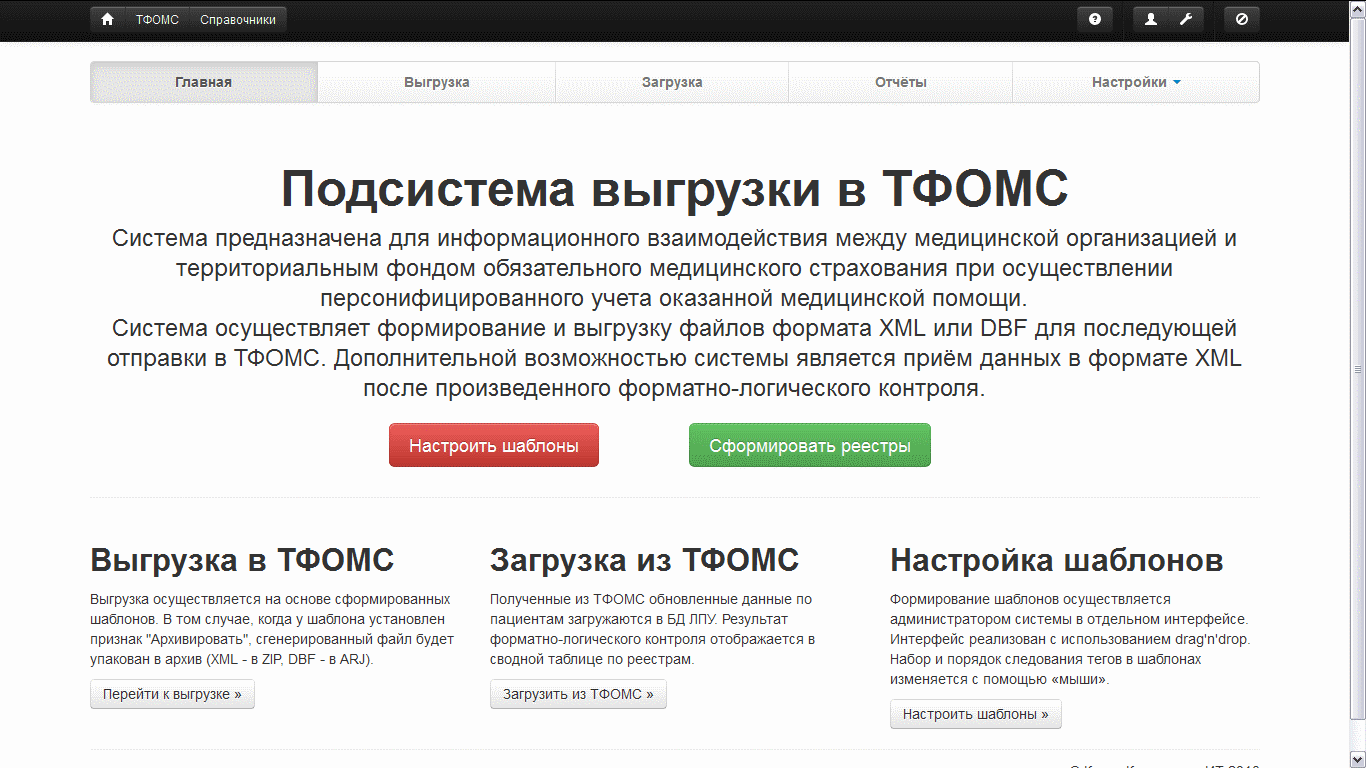
\includegraphics[width = 1\textwidth ,keepaspectratio]{tfoms_main}
 \caption{Главная страница подсистемы выгрузки в ТФОМС}
 \label{img_tfoms_main}
\end{figure} 

\subsection{Выгрузка}

В данном разделе подсистемы осуществляется выгрузка данных о пролеченных пациентах и их обращениях для последующей передачи в ТФОМС.

Для перехода в данный раздел (Рисунок \ref{img_tfoms_unload}) необходимо нажать кнопку \btn{Выгрузка} в верхней части любой страницы подсистемы либо нажать кнопку \btn{Cформировать реестры}  или \btn{Перейти к выгрузке}  на главной странице подсистемы.

\begin{figure}[ht]\centering
 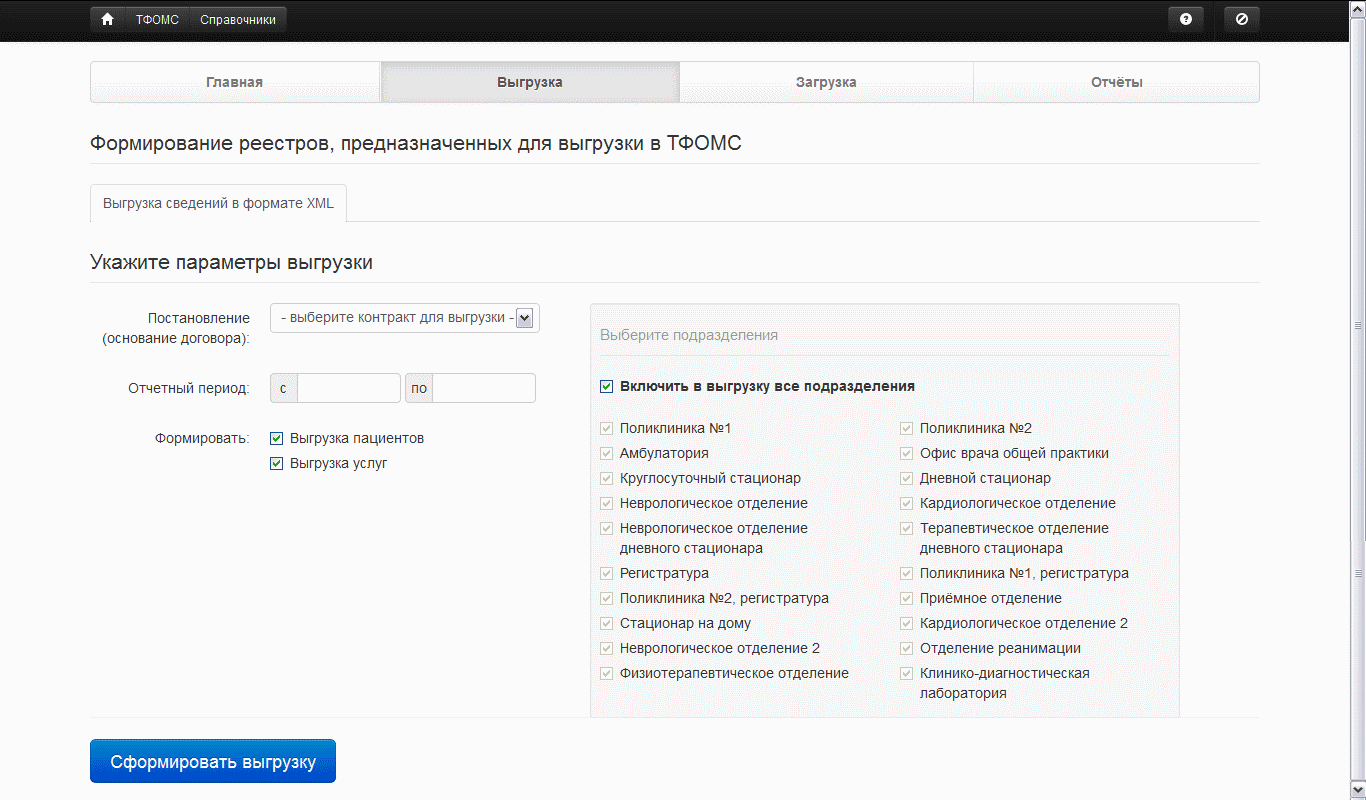
\includegraphics[width = 1\textwidth ,keepaspectratio]{tfoms_unload}
 \caption{Раздел <<Выгрузка>> подсистемы выгрузки в ТФОМС}
 \label{img_tfoms_unload}
\end{figure}

Для осуществления выгрузки необходимо:
\begin{enumerate}
 \item Выбрать вкладку, соответствующую требуемому формату выгрузки.
 \item Указать параметры выгрузки (см. ниже).
 \item Нажать кнопку \btn{Сформировать выгрузку}.
\end{enumerate}

При выгрузке задаются следующие параметры:
\begin{itemize}
 \item \dm{Постановление (основание договора)} – выбирается из списка основание договора (источник финансирования), по которому будет осуществляться выгрузка.
 item \dm{Отчетный период} – период, за который следует выгружать данные о случаях обращения. Указываются начальная и конечная дата периода. Даты заполняются вручную с клавиатуры или выбираются из календаря. Календарь раскрывается автоматически при установке курсора в поле даты.
 \item При установке флажка \dm{Выгрузка пациентов} будет осуществляться выгрузка персональных данных пациентов, получивших медицинскую помощь в указанный период.
 \item При установке флажка \dm{Выгрузка услуг} будет осуществляться выгрузка сведений о случаях обращений пациентов за медицинской помощью в указанный период.
 \item В блоке выбора подразделения можно выбрать отдельные отделения, по которым необходимо выполнить выгрузку. При установке флажка \dm{Включить в выгрузку все подразделения}, флажки устанавливаются автоматически для всех перечисленных подразделений, а редактирование их становится невозможным. Для того чтобы снова иметь возможность выбора подразделений, следует снять флажок \dm{Включить в выгрузку все подразделения}.
\end{itemize}
 
Формирование выгрузки может занять продолжительное время. Во время подготовки данных на экране будет отображаться страница ожидания (Рисунок \ref{img_tfoms_unload_proc}).

\begin{figure}[ht]\centering
 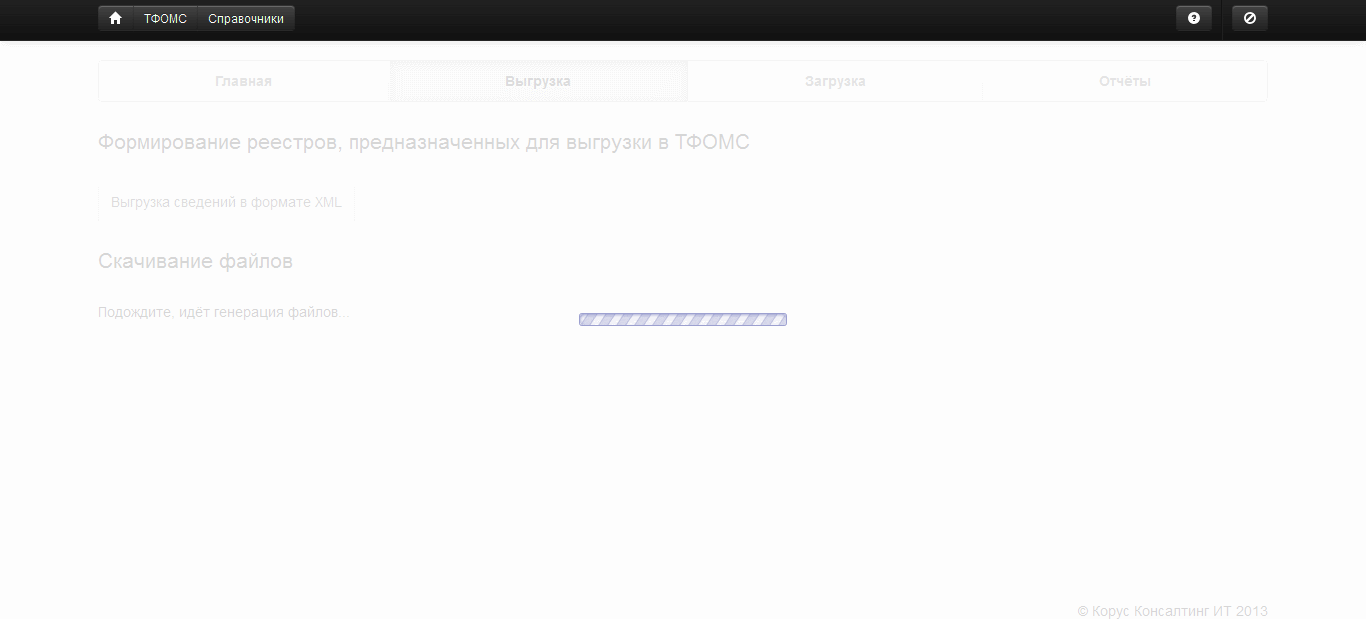
\includegraphics[width = 1\textwidth ,keepaspectratio]{tfoms_unload_proc}
 \caption{Выполнение выгрузки}
 \label{img_tfoms_unload_proc}
\end{figure}

После того как файлы выгрузки будут сформированы, они станут доступны для скачивания. Для скачивания файла необходимо щелкнуть по нему левой кнопкой мыши, в появившемся окне выбрать Сохранить и нажать кнопку \btn{OK}, а затем указать папку для сохранения.

В зависимости от настроек шаблона выгрузки файлы могут быть выгружены в заархивированном (ZIP, ARJ) или распакованном виде.

\subsection{Загрузка}

В данном разделе подсистемы осуществляется загрузка данных об отклоненных случаях обращений по результатам проверки в ТФОМС для ранее выгруженных данных.

\begin{vnim}
 Загрузка данных возможна только в формате XML
\end{vnim}

Для перехода в данный раздел (Рисунок \ref{img_tfoms_upload}) необходимо нажать кнопку \btn{Звгрузка}  в верхней части любой страницы подсистемы либо нажать кнопку \btn{Загрузить из ТФОМС >>}  на главной странице подсистемы.

\begin{figure}[ht]\centering
 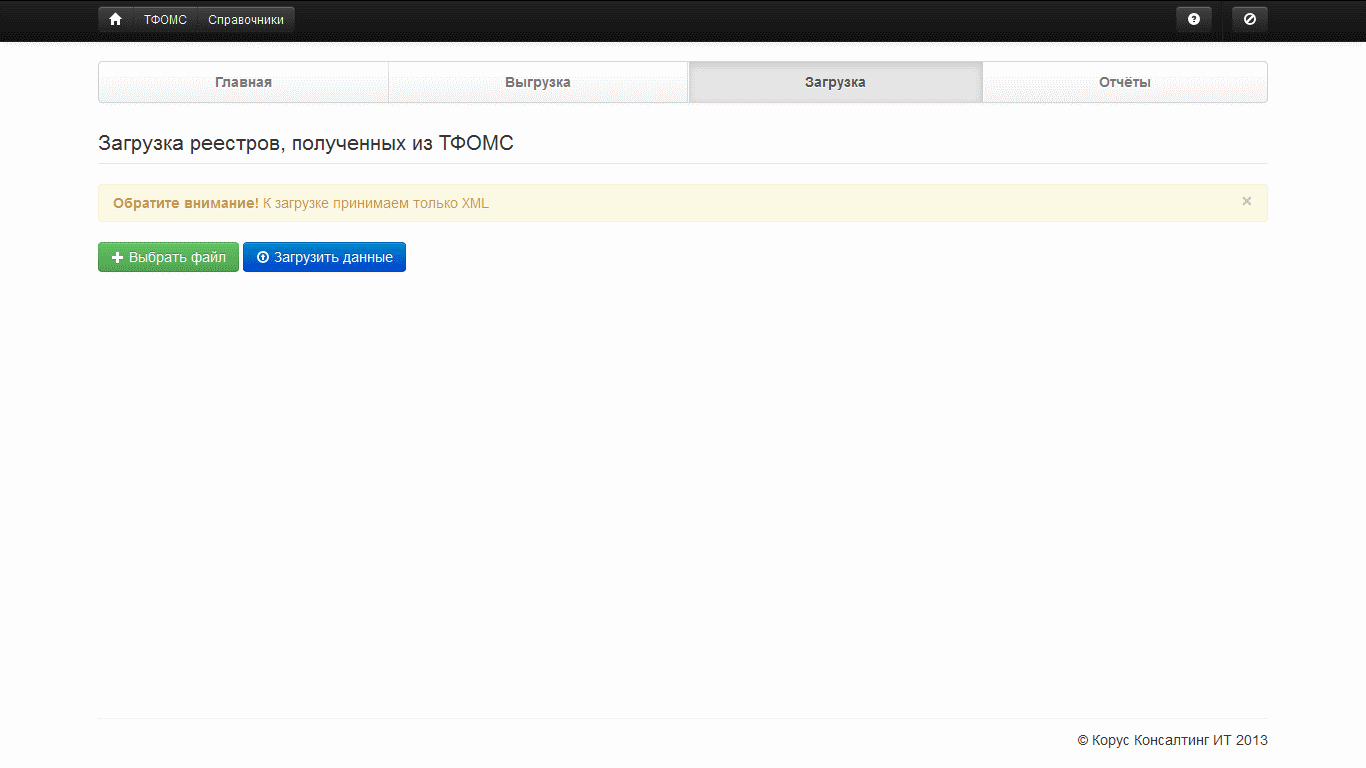
\includegraphics[width = 1\textwidth ,keepaspectratio]{tfoms_upload}
 \caption{Раздел <<Загрузка>> подсистемы выгрузки в ТФОМС}
 \label{img_tfoms_upload}
\end{figure}

Для загрузки результатов проверки ранее выгруженных файлов необходимо нажать на кнопку \btn{Выбрать файл}, в открывшемся окне перейти в нужную папку и выбрать файл для загрузки. После выбора файла его имя появится под кнопкой \btn{Выбрать файл}. Далее необходимо нажать кнопку \btn{Загрузить данные}. После непродолжительного ожидания на странице появится сообщение о результатах загрузки (Рисунок \ref{img_tfoms_upload_rez}).

\begin{figure}[ht]\centering
 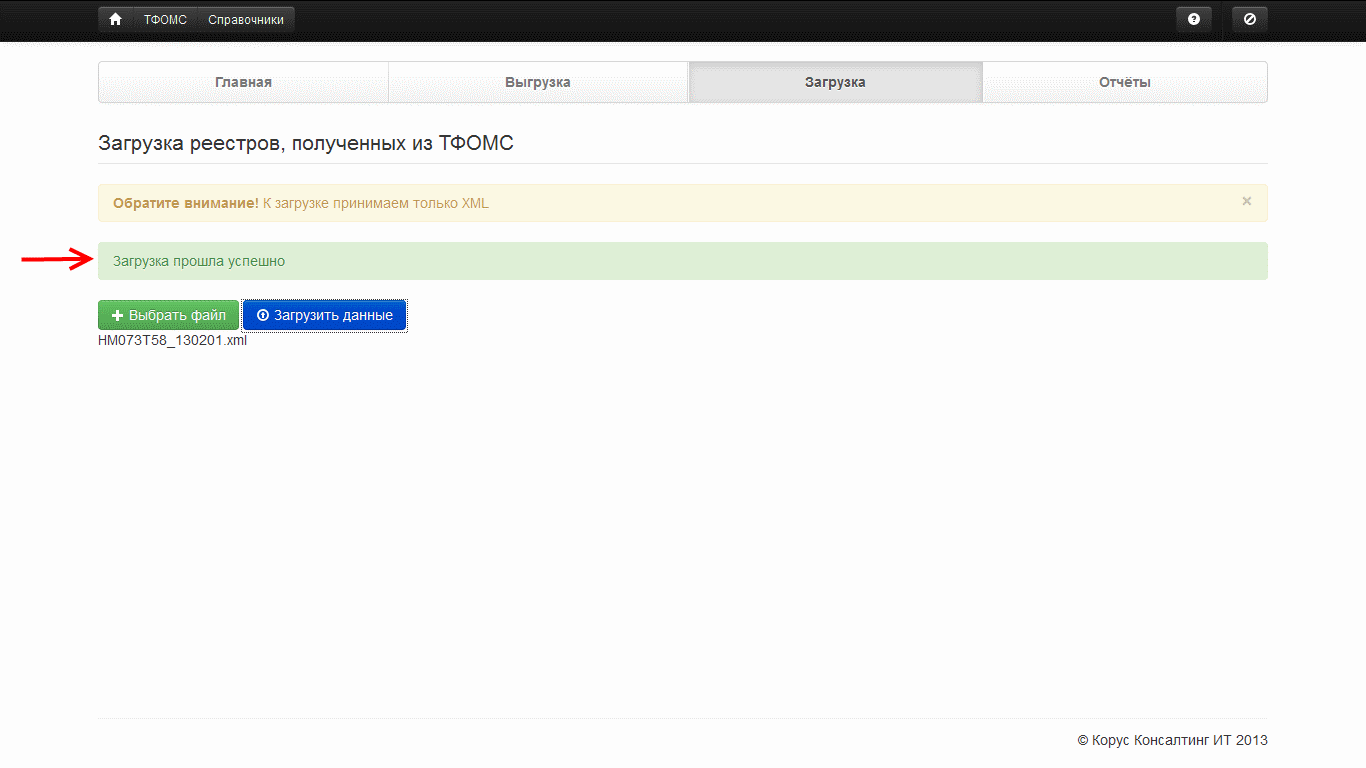
\includegraphics[width = 1\textwidth ,keepaspectratio]{tfoms_upload_rez}
 \caption{Результат загрузки файла}
 \label{img_tfoms_upload_rez}
\end{figure}

\subsection{Отчеты}

В разделе \dm{Отчеты} хранится история выполненных выгрузок. По любой из выгрузок можно просмотреть позиции, попавшие в счет и повторно скачать файлы, полученные в результате выгрузки.

Для перехода в данный раздел (Рисунок \ref{img_tfoms_rep}) необходимо нажать кнопку \btn{Отчеты}  в верхней части любой страницы подсистемы. Список всех выгрузок в ТФОМС будет представлен в виде таблицы.

\begin{figure}[ht]\centering
 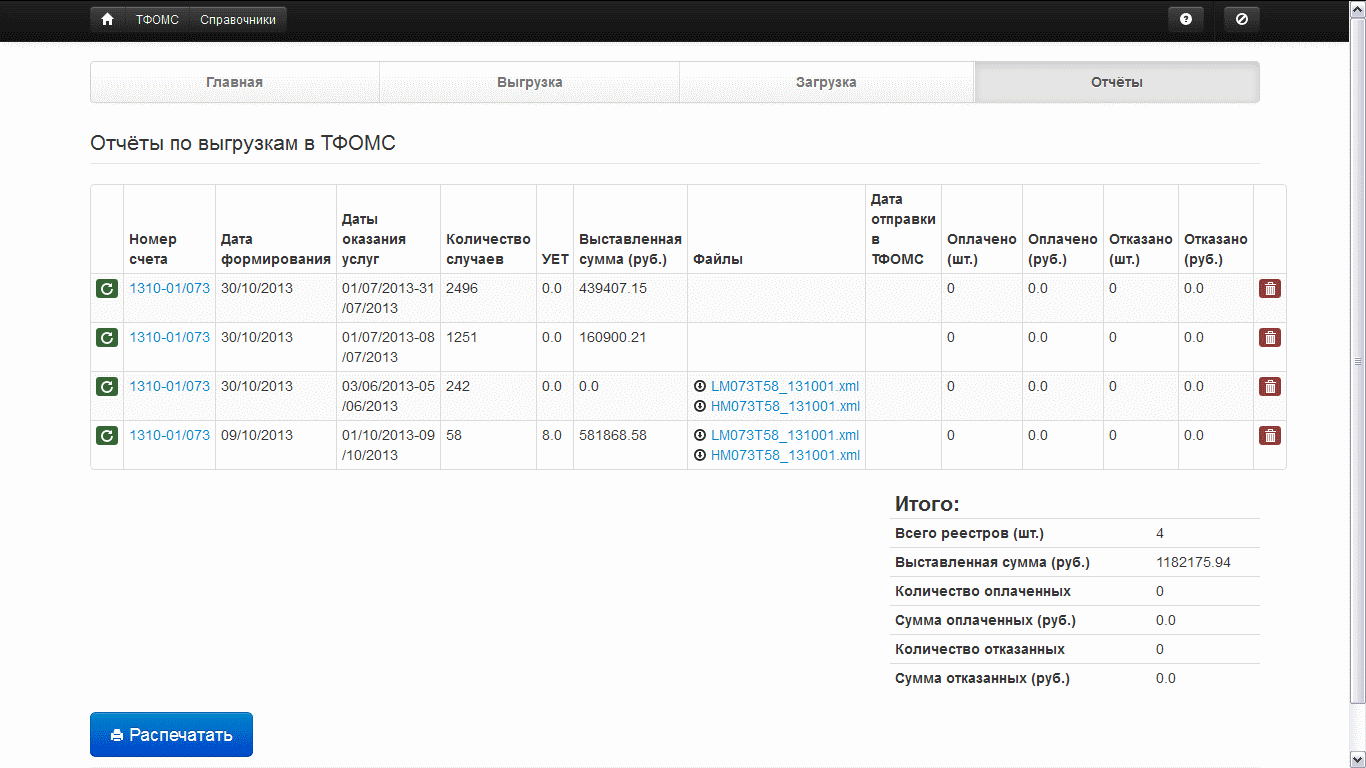
\includegraphics[width = 1\textwidth ,keepaspectratio]{tfoms_rep}
 \caption{Раздел <<Отчеты>> подсистемы выгрузки в ТФОМС}
 \label{img_tfoms_rep}
\end{figure}

Кнопка 
\includegraphics{re} позволяет сформировать выбранную выгрузку еще раз. При ее нажатии осуществляется автоматический переход в раздел \dm{Выгрузки}, а параметры выгрузки устанавливаются такими же, как при текущей выгрузке. При необходимости можно изменить параметры. Для запуска повторной выгрузки следует нажать кнопку \btn{Сяормировать выгрузку}. После ее завершения в список отчетов добавится новая строка.

Кнопка 
\includegraphics{del}  позволяет удалить выбранный отчет. После нажатия на нее необходимо подтвердить удаление в появившемся окне (Рисунок \ref{img_tfoms_rep_del}).

\begin{figure}[ht]\centering
 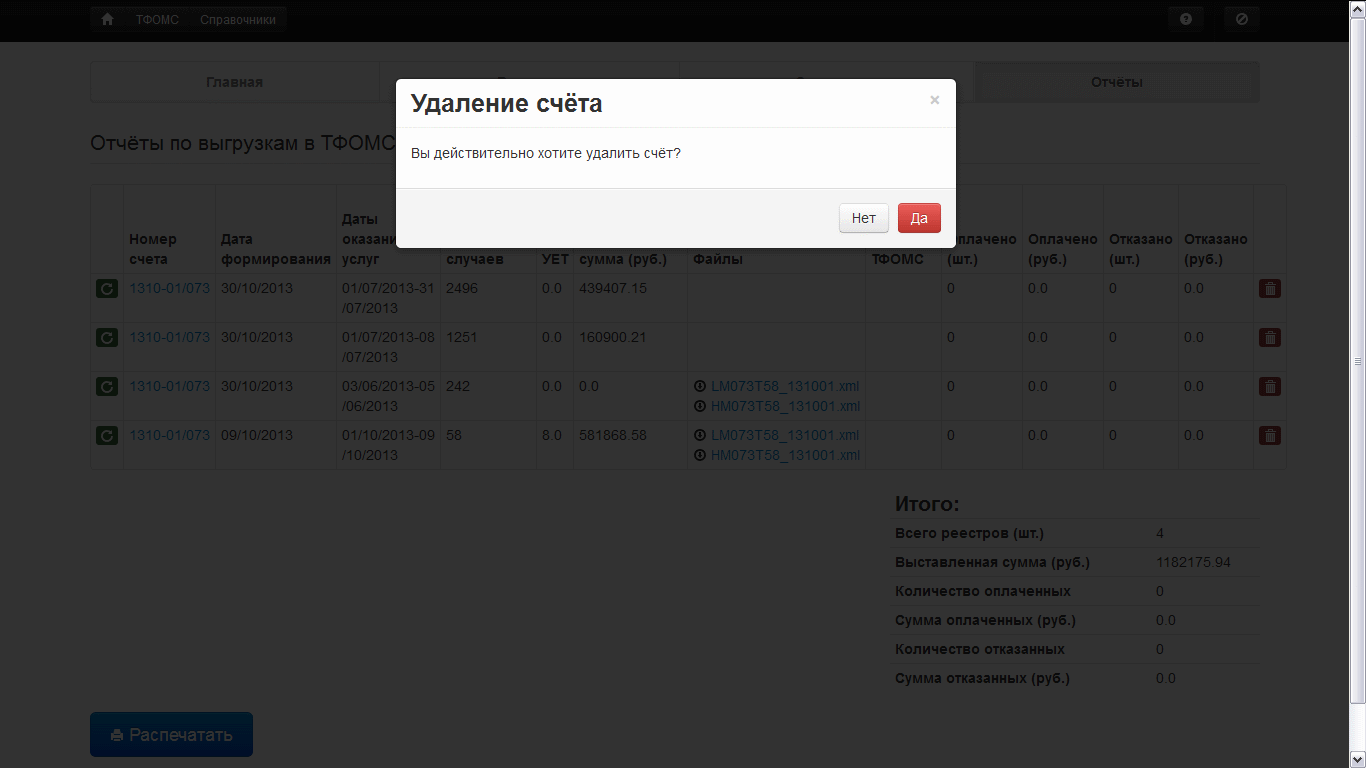
\includegraphics[width = 1\textwidth ,keepaspectratio]{tfoms_rep_del}
 \caption{Подтверждение удаления отчета}
 \label{img_tfoms_rep_del}
\end{figure}

Таблица отчетов содержит следующую информацию:
\begin{itemize}
 \item \dm{Номер счета} – номер счета, под которым результаты выгрузки передаются в ТФОМС. При нажатии левой кнопкой мыши на номер счета, открывается страница, содержащая список случаев, попавших в выбранную выгрузку.
 \item \dm{Дата формирования} – дата формирования выгрузки.
 \item \dm{Даты оказания услуг} – период, за который осуществлялась выгрузка.
 \item \dm{Количество случаев} – количество случаев обращений, попавших в данную выгрузку.
 \item \dm{УЕТ} – суммарное количество УЕТ по всем случаям, попавшим в выгрузку.
 \item \dm{Выставленная сумма (руб.)} – общая стоимость услуг по всем случаям, попавшим в выгрузку.
 \item \dm{Файлы} – названия файлов, полученных в результате выгрузки. При нажатии левой кнопкой мыши на имя файла, его можно сохранить в выбранную папку на компьютере.
 \item \dm{Дата отправки в ТФОМС} – проставляется после загрузки результатов проверки из ТФОМС.
 \item \dm{Оплачено (шт.)} – количество оплаченных случаев обращения. Данные будут отображаться после загрузки результатов проверки данной выгрузки, полученных из ТФОМС.
 \item \dm{Оплачено (руб.)} – общая стоимость услуг по всем оплаченным случаям обращения. Данные будут отображаться после загрузки результатов проверки данной выгрузки, полученных из ТФОМС.
 \item \dm{Отказано (шт.)} – количество отклоненных случаев по результатам проверки ТФОМС. Данные будут отображаться после загрузки результатов проверки данной выгрузки, полученных из ТФОМС.
 \item \dm{Отказано (руб.)} – общая стоимость услуг по всем отказанным случаям обращения. Данные будут отображаться после загрузки результатов проверки данной выгрузки, полученных из ТФОМС.
\end{itemize}
 
В низу страницы отображается сводная информация по всем выгрузкам.